

% ===========================
\chapter{Ergebnis}
\label{ergebnis}
% ===========================

In diesem Kapitel werden die Ergebnisse der trainierten \acp{KNN} aus Abschnitt \ref{umsetzung_training_architektur} mit den Parametern aus Abschnitt \ref{umsetzung_training_experimente} vorgestellt. Jede Architektur wird mit einer Maximalanzahl von 100 Epochen trainiert. Aufgrund der Regularisierungsmethode Early Stopping wird diese Anzahl jedoch nie erreicht. Das Training bricht jeweils ab, wenn sich die Klassifizierungsgenauigkeit der Validierungsdaten innerhalb von 20 Epochen nicht um mindestens 0,01 verbessert. Nach Abbruch werden jeweils die Gewichte der Epoche mit der höchsten Validierungsgenauigkeit wiederhergestellt. 

In Abschnitt \ref{ergebnis_parameter} wird die Genauigkeit der jeweiligen Netzarchitekturen bei der Klassifizierung von realen Testdaten und die Anzahl der trainierten Epochen hinsichtlich der unterschiedlichen Parameter aus Abschnitt \ref{umsetzung_training_experimente} verglichen. Danach wird in Abschnitt \ref{ergebnis_synth_vs_real} die Genauigkeit der Klassifizierung zwischen realen und synthetischen Testdaten untersucht. Im Anschluss werden in Abschnitt \ref{ergebnis_szenarien} die Unterschiede bei der Erkennung von verschiedenen Klassen erörtert.

% ===========================
\section{Variation der Parameter}
\label{ergebnis_parameter}
% ===========================

In diesem Abschnitt werden die Unterschiede der verschiedenen Architekturen aus Abschnitt \ref{umsetzung_training_architektur} noch einmal kurz aufgegriffen und dann die dazugehörigen Ergebnisse vorgestellt. Die Ergebnisse sind in Tabelle \ref{tab_ergebnis_real} zusammengefasst.

\begin{table}[h]
\small
\centering
\def\arraystretch{1.4}
\begin{tabular}{c p{3cm} c c}
\textbf{Architektur} & \textbf{Beschreibung} & \textbf{Genauigkeit} & \textbf{Epochen} \\
\hline
A & Inception-V3 & 0,73 & 4 \\
\hline
B & Inception-V3 \newline Dropout & 0,64 & 1 \\
\hline
C & Xception & 0,54 & 1 \\
\hline
D & Xception \newline Dropout & 0,48 & 9 \\
\hline 
E & Inception-V3 \newline LSTM & 0,36 & 80 \\
\hline
F & Inception-V3 \newline LSTM \newline Dropout & 0,95 & 12 \\
\hline
G & Xception \newline LSTM & 0,38 & 26 \\
\hline
H & Xception \newline LSTM \newline Dropout & 0,61 & 9 \\
\hline
\end{tabular}
\caption{Ergebnisse der verschiedenen Architekturen bei der Klassifizierung der realen Testdaten}
\label{tab_ergebnis_real}
\end{table}

% ===========================
\subsubsection{Prinzip der Klassifizierung}
% ===========================

Bei dem Prinzip der Klassifizierung wird in dieser Arbeit zwischen \acp{KNN} für die Erkennung von einzelnen Bildern und für die Erkennung von 3-Sekunden-Videos mit jeweils 15 Bildern unterschieden. Die detaillierten Architekturen sind in Abschnitt \ref{umsetzung_training_architektur} vorgestellt.

Insgesamt wird die höchste Genauigkeit bei der Klassifizierung von realen Testdaten von 0,95 mit der Architektur F für Videoerkennung erreicht. Das Ergebnis dieser Architektur nach einzelnen Klassen ist auch in Abbildung \ref{fig_cm_v3_lstm_d_real} in der Konfusionsmatrix (engl. confusion matrix) dargestellt. Auf die Unterschiede der Genauigkeiten zwischen den einzelnen Klassen wird in Abschnitt \ref{ergebnis_szenarien} genauer eingegangen. Die niedrigste Genauigkeit von 0,28 wird mit der Architektur H für Videoerkennung erreicht. Architekturen für die reine Bilderkennung erreichen Genauigkeiten zwischen 0,48 (Architektur D) und 0,73 (Architektur A). Damit erzielen diese Architekturen Ergebnisse mit weniger Varianz im Vergleich zu den Architekturen mit \ac{LSTM}-Schicht. Eine Erklärung hierfür kann die niedrigere Komplexität der \acp{KNN} sein. Bei einer höheren Komplexität, also mehr trainierbaren Parametern, kann es sein, dass die Genauigkeiten zwischen verschiedenen Architekturen stärker schwankt, weil mehr Parameter für die richtige Klassifizierung benötigt werden.

\begin{figure}[h]
\centering
{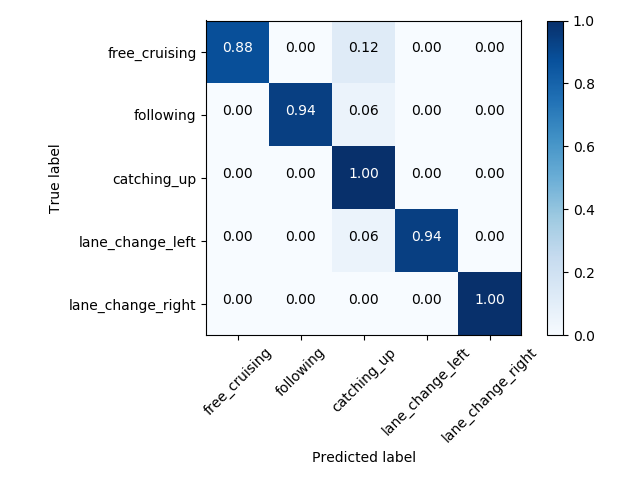
\includegraphics[scale=0.7]{images/cm_v3_lstm_d_real.png}}
\caption{Konfusionsmatrix der Klassifizierung von realen Testdaten mit der Architektur F (Inception-V3, \ac{LSTM}, Dropout)}
\label{fig_cm_v3_lstm_d_real}
\end{figure}

% ===========================
\subsubsection{\aclp{CNN}}
% ===========================

Der Vergleich zwischen den zwei \ac{CNN}-Architekturen Inception-V3 und Xception zeigt ein klares Bild. In drei von vier Fällen kann die Architektur mit der Inception-V3-Architektur als Basis bessere Ergebnisse erzielen. Die Differenz bei der Genauigkeit liegt dabei zwischen 0,16 und 0,67. Nur die Architektur G erzielt eine höhere Genauigkeit als Architektur E mit einem Unterschied von 0,02. Dieser Unterschied überrascht, da die Xception-Architektur in anderen Arbeiten \cite{chollet2017xception} höhere Genauigkeiten bei der Klassifizierung von Bildern erreicht hat.

% ===========================
\subsubsection{Regularisierung mit Dropout}
% ===========================

Es ist auffällig, dass die Architekturen für Videoklassifizierung mit Dropout in der vorletzten Fully-Connected-Schicht deutlich bessere Ergebnisse erzielen können im Vergleich zu denselben Architekturen ohne Dropout. Im Gegensatz dazu erzielen die Architekturen für die Erkennung einzelner Bilder die besseren Genauigkeit ohne Regularisierung mit Dropout in der vorletzten Schicht. Die Erklärung kann auf die Grundidee von Dropout zurückgeführt werden. Dropout ist eine Methode um die Komplexität eines \acp{KNN} während dem Training zu reduzieren. Daher hat Dropout einen sehr positiven Effekt auf die Architekturen für Videoklassifizierung, die mit der \ac{LSTM}-Schicht deutlich komplexer sind, also mehr Parameter besitzen, als die Architekturen für Bildklassifizierung.

In Abbildung \ref{fig_acc_v3_lstm} ist beispielhaft die Entwicklung der Genauigkeit der Trainings- und Testdaten während dem Training von den Architekturen E und F dargestellt. Es ist deutlich zu sehen, dass die Anzahl der Epochen bei Architekturen mit \ac{LSTM}-Schicht mit Dropout stark reduziert werden kann und die Genauigkeit weniger sprunghaft ist und schneller konvergiert.

\begin{figure}[h]
\centering
\begin{tabular}{cc}
\subfloat[Architektur E (Inception-V3, LSTM)]{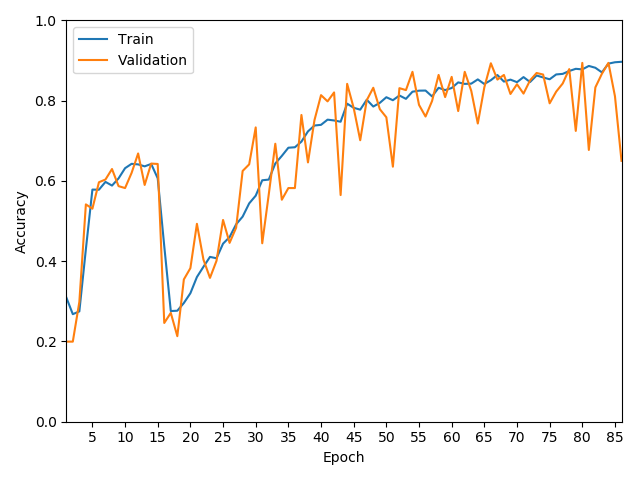
\includegraphics[scale=0.4]{images/acc_v3_lstm_86.png}} &
\subfloat[Architektur F (Inception-V3, LSTM, Dropout)]{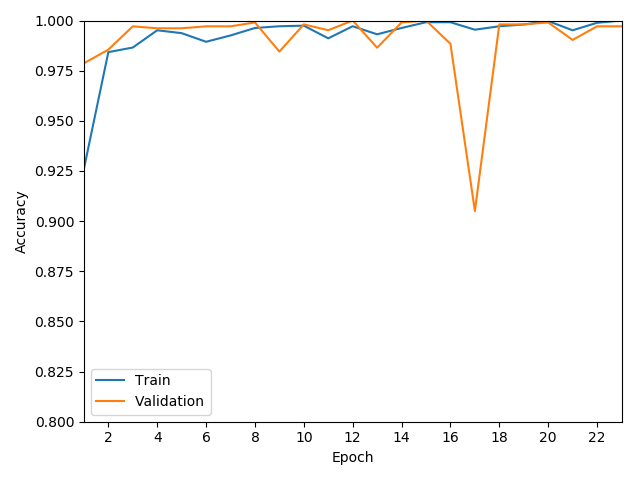
\includegraphics[scale=0.4]{images/acc_v3_lstm_dropout_23.png}}
\end{tabular}
\caption{Genauigkeit der Trainings- und Testdaten während dem Training von zwei verschiedenen Architekturen}
\label{fig_acc_v3_lstm}
\end{figure}

Eine Erklärung dafür ist die Komplexität der Architekturen mit \ac{LSTM}-Schicht. Diese Architekturen haben mehr trainierbare Parameter und sind daher anfälliger für eine Überanpassung \cite{hinton2012improving}. Dropout reduziert die Anzahl der Parameter und damit die Komplexität, was zu weniger benötigten Trainingsschritten und einer schnelleren Konvergenz der Gewichtsanpassung führt. Die Architekturen mit reinen \acp{CNN} sind weniger komplex und daher hat Dropout keine oder eine negative Auswirkung auf das Ergebnis.

% ===========================
\subsubsection{Anzahl der Epochen}
% ===========================

Es lässt sich beobachten, dass die Architekturen für die Klassifizierung von Videos mit bis zu 86 Epochen deutlich mehr Trainingsschritte benötigen als die Architekturen für reine Bilderkennung. Eine mögliche Erklärung dafür ist, dass reine \acp{CNN} eine weniger komplexe Architektur und weniger Parameter haben als die Architekturen mit einer \ac{LSTM}-Schicht. Mehr Gewichte, die angepasst werden können, bedeutet eine höhere Komplexität und dementsprechend mehr benötigte Epochen.

Zu den Unterschieden der Epochenanzahl zwischen der Inception-V3- und der Xception-Architektur lässt sich in dieser Arbeit keine eindeutige Aussage treffen. Die benötige Epochenanzahl bei beiden Architekturen variiert sehr stark.

% ===========================
\section{Synthetische und reale Testdaten}
\label{ergebnis_synth_vs_real}
% ===========================

\begin{table}[h]
\small
\centering
\def\arraystretch{1.4}
\begin{tabular}{c p{3cm} c c}
\textbf{Architektur} & \textbf{Beschreibung} & \textbf{Genauigkeit} & \textbf{Genauigkeit} \\
 & & \textbf{Reale Testdaten} & \textbf{Synthetische Testdaten} \\
\hline
A & Inception-V3 & 0,73 & 0,96 \\
\hline
B & Inception-V3 \newline Dropout & 0,64 & 0,96 \\
\hline
C & Xception & 0,54 & 0,2 \\
\hline
D & Xception \newline Dropout & 0,48 & 0,36 \\
\hline 
E & Inception-V3 \newline LSTM & 0,36 & 0,94 \\
\hline
F & Inception-V3 \newline LSTM \newline Dropout & 0,95 & 0,99 \\
\hline
G & Xception \newline LSTM & 0,38 & 0,99 \\
\hline
H & Xception \newline LSTM \newline Dropout & 0,61 & 0,91 \\
\hline
\end{tabular}
\caption{Ergebnisse der Klassifizierung von synthetischen und realen Testdaten}
\label{tab_ergebnis_synth}
\end{table}

In diesem Abschnitt werden die Unterschiede der Genauigkeiten bei der Klassifizierung zwischen realen und synthetischen Testdaten untersucht. Die Ergebnisse sind in Tabelle \ref{tab_ergebnis_synth} zusammengefasst. Es ist nicht überraschend, dass die Genauigkeiten bei der Klassifizierung von synthetischen Testdaten überwiegend deutlich höher ist, weil die \acp{KNN} mit 95\% synthetischer und nur 5\% realer Daten trainiert wurden. Das bestätigt auch die Ergebnisse der vorangegangenen Arbeit, die in Abschnitt \ref{grundlagen_nn_synthetisch} diskutiert werden. 

Es ist auffällig, dass die Klassifizierung von einzelnen synthetischen Bildern mit der Xception Architektur niedriger ist als die Klassifizierung von realen Testbildern. Aktuell hat der Autor keine Erklärung hierfür. Dieses Ergebnis kann als Ausgangspunkt für weitere Untersuchungen dienen.


% ===========================
\section{Genauigkeit der einzelnen Szenarien}
\label{ergebnis_szenarien}
% ===========================

Die Betrachtung von Klassifizierungsgenauigkeiten der einzelnen Klassen ergibt kein eindeutiges Bild. Bei verschiedenen Architekturen werden verschiedene Szenen teilweise besser oder schlechter erkannt. Hervorzuheben ist, dass es deutliche Unterschiede gibt, diese aber keinem erkennbaren Muster folgen. Eine Übersicht der Genauigkeit der Klassifizierung von realen Testdaten auf der Ebene von Szenarienklassen ist in Tabelle \ref{tab_ergebnis_szenarien} dargestellt.

Ausgehend von der Architektur mit der höchsten Gesamt-Genauigkeit, Architektur F, kann man die folgenden Überlegungen zu unterschiedlichen Genauigkeiten zwischen Klassen anstellen. Bei Architektur F wurden die Klassen \textit{catching up} und \textit{lane change left} sehr gut erkannt. Die Klasse \textit{free cruising} wurde am schlechtesten erkannt. Da die Erkennung auf reinen Bilddaten basiert, kann argumentiert werden, dass Szenenarien der Klasse \textit{free cruising} den Szenarien aus den Klassen \textit{following} und \textit{catching up} ähneln, weil der Unterschied nur im Abstand zu anderen Fahrzeuge liegt. Dagegen sind die Klassen \textit{lane change left} und \textit{lane change right} eindeutiger, weil jeweils die Fahrbahnmarkierung überquert wird und damit ein eideutigeres Merkmal existiert. Diese Erklärung ist aktuell allerdings nur eine mögliche Interpretation des Autors und kann bisher nicht weiter belegt werden. 

\begin{table}[h]
\small
\centering
\def\arraystretch{1.4}
\begin{tabular}{c c c c c c}
\textbf{Architektur} & \textbf{Free} & \textbf{Following} & \textbf{Catching} & \textbf{Lane change} & \textbf{Lane change} \\
 & \textbf{cruising} & & \textbf{up} & \textbf{left} & \textbf{right} \\
\hline
A & 0,65 & 0,76 & 1,00 & 0,35 & 0,88 \\
B & 0,94 & 0,47 & 0,88 & 0,29 & 0,59 \\
C & 0,76 & 0,94 & 0,94 & 0,00 & 0,06 \\
D & 0,00 & 0,82 & 0,82 & 0,76 & 0,00 \\
E & 0,59 & 0,47 & 0,41 & 0,06 & 0,29 \\
F & 0,88 & 0,94 & 1,00 & 0,94 & 1,00 \\
G & 0,47 & 0,06 & 0,18 & 0,59 & 0,06 \\
H & 0,71 & 1,00 & 0,71 & 0,35 & 0,29 \\
\hline
\textbf{Durchschnitt} & 0,62 & 0,68 & 0,74 & 0,42 & 0,40 \\
\hline
\end{tabular}
\caption{Genauigkeit der Klassifizierung von realen Testdaten auf der Ebene von Szenarienklassen}
\label{tab_ergebnis_szenarien}
\end{table}

Um an dieser Stelle besser verstehen zu können auf welcher Basis die \acp{KNN} die Bilder und Bildsequenzen erkennen, sollten in nachfolgenden Arbeiten weitere Untersuchungen dazu angestellt werden. So wäre es beispielsweise interessant, welche Teile der einzelnen Bilder stärker oder auch weniger stark bei der Klassifizierung berücksichtigt werden.








